
\chapter{LEGO MINDSTORMS NXT}
I dette kapitel vil den valgte platform, \legoms, blive kort beskrevet, samt en begrundelse for dette valg.
Yderligere vil der blive argumenteret for valg af API til NXT-enheden.

\section{Hvad er LEGO MINDSTORMS?}
\legoms er et byggesæt, hvor det er muligt at bygge programmerbare robotter(her menes også andre maskiner der måske ikke altid vil blive betegnet som robotter) i \lego-klodser.

Til at bygge disse robotter er der i \legoms nogle sensorer og aktuatorer. Sensorerne gør det muligt for robotten at modtage input fra sine omgivelser og ved brug af aktuatorerne kan robotten reagere på disse.

Ud over de originale \lego dele er der også tredjeparts forhandlere, som har et udbud af andre sensorer og aktuatorer.

\subsection{Hvad er NXT?}
Denne sektion er baseret på \cite{nxt}, hvilket omhandler NXT 2.0, som er den version der bruges i dette projekt.
NXT Intelligent Brick (oftest kaldt blot 'NXT' eller 'brick') er hjernen i \legoms robotten.
Det er den der står for at modtage og behandle input fra sensorer, samt at styre aktuatorer.
Et billede af NXT 2.0 kan ses i \cref{platform:nxt}.

\begin{figure}
\begin{center}
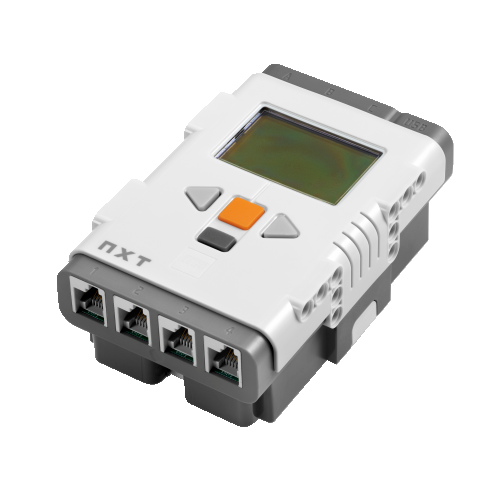
\includegraphics[scale=.5]{./graphics/nxt/brick}
\end{center}
\caption{'NXT Intelligent Brick'}
\label{platform:nxt}
\end{figure}

\subsubsection{Porte}
NXT'en har 3 motor porte (kaldet A, B og C) og 4 sensor porte (kaldet 1, 2, 3 og 4).

\subsubsection{Tilslutningsmuligheder}
Der kan kommunikeres med NXT'en ved at tilslutte den til en anden enhed med USB-kabel eller Bluetooth\textregistered.

\subsubsection{Feedback}
Til output har NXT'en en 100 x 64 pixel LCD display samt en 8 kHz højttaler.

\subsubsection{Styring}
NXT'en kan styres på to måder:
Man kan sende kommandoer og modtage beskeder (for eksempel sensor aflæsninger) på en ekstern enhed (oftest en computer eller en anden NXT).
Alternativt kan programmer sendes (via Bluetooth eller USB) til NXT'en, hvorfra de kan køres direkte på NXT'en, uafhængig af eksterne enheder.

Til at styre NXT'en kan bruges et væld af programmeringssprog.
Yderligere er det også muligt at erstatte den originale firmware med en brugerdefineret, hvilket giver endnu flere muligheder.
Kombination af firmware og programmeringssprog (samt eventuelle værktøjer) er hvad vi betragter som et API.
De forskellige API'er samt vores valg af API diskuteres i \cref{nxt_api}.

\subsubsection{Tekniske specifikationer}
De tekniske specifikationer for NXT 2.0:\cite{nxt}
\begin{itemize}
\item{32-bit ARM7 microcontroller}
\item{256 Kb FLASH, 64 Kb RAM}
\item{8-bit AVR controller}
\item{4 Kb FLASH, 512 b RAM}
\item{Bluetooth wireless communication (Bluetooth Class II V2.0 compliant)}
\item{USB full speed port (12 Mbit/s)}
\item{4 input ports, 6-wire cable digital platform (One port includes a IEC 61158 Type 4/EN 50 170 compliant expansion port for future use)}
\item{3 output ports, 6-wire cable digital platform}
\item{100 x 64 pixel LCD graphical display}
\item{Loudspeaker - 8 kHz sound quality. Sound channel with 8-bit resolution and 2-16 kHz sample rate}
\item{Power source: 6 AA batteries}
\end{itemize}

\section{Hvorfor LEGO MINDSTORMS NXT?}
Der er mange gode grunde til at vælge \legoms NXT.
Her er givet fire overordnede punkter, der vil blive gennemgået efterfølgende:

\begin{itemize}
\item{Tilgængelighed}
\item{Nemt at gå til}
\item{Stort udvalg af sensorer}
\item{Mange muligheder ift. styring}
\end{itemize}

\subsubsection{Tilgængelighed}
Grundet at \lego (inkl. \legoms) er ment til almindelige brugere, er det masseproduceret og kan derved købes forholdsvist billigt og i helt almindelige butikker (legetøjsforretninger og ofte også supermarkeder).

\subsubsection{Nemt at gå til}
Det faktum at man bygger sin robot i \lego klodser, med tilføjelse af \legoms sensorer/aktuatorer, gør at det i første gang er nemt at lave en konstruktion.
Samtidig er det også nemt at tilpasse en tidligere konstruktion, ved at tilføje/flytte/fjerne klodser eller sensorer/aktuatorer.

Denne høje versatilitet gør at \lego er perfekt til en prototype-orienteret fremgangsmåde.

\subsubsection{Stort udvalg af sensorer}
Det store udvalg af sensorer gør at der kan bygges robotter der kan løse et væld af opgaver.
Ved et projekt med høj usikkerhed, er det derved også nemt og billigt at udskifte en sensor med en mere passende.

\subsubsection{Mange muligheder ift. styring}
Her menes der både overordnet den måde hvorpå robotten styres, men især også den måde hvorpå NXT'en styres.
Som nævnt tidligere kan NXT'en udstyres med brugerdefineret firmware, der gør at der er utroligt mange muligheder ift. styring af den.
Desuden kan der bruges et væld af programmeringssprog til at programmere NXT'en.
Der vil blive gået mere i dybden med de forskellige muligheder ift. API i \cref{nxt_api}.


\section{Valg af NXT API}
\label{nxt_api}

I denne sektion vil der blive argumenteret for valg af API.
Først vil de forskellige afprøvede API'er blive kort præsenteret, hvorefter vores valg vil blive fremhævet.

Overordnet set er der to muligheder når det kommer til valg af API; standard eller custom firmware.
Forskellene på de to og hvilke mulige sprog/API'er der er indenfor de to vil blive uddybet her.

\subsection{Standard firmware}
Ens for alle API'er der benytter sig af standard firmware, er at de sender kommandoer til at styre NXT'en.
Derved er det nemt at lave et bibliotek/interface til at styre NXT'en, hvilket også er derfor der er mange muligheder til valg af sprog.

Følgende NXT platforme som benytter sig af standard firmware er blevet undersøgt:
\begin{itemize}
\item{nxt-python}
\item{Mindsqualls}
\item{ROBOTC}
\end{itemize}

\paragraph{nxt-python} er et Python interface der gør det muligt at sende kommandoer direkte til NXT'en.
For at bruge Bluetooth\textregistered til at kommunikere med NXT'en, skal der bruges et eksternt bibliotek.\cite{nxt-python}

\paragraph{Mindsqualls} er et .NET bibliotek, der gør det muligt at programmere til NXT'en i Common Language Interface (CLI) sprog, som \csharp, \fsharp eller VB.\cite{mindsqualls}

Yderlige kan der ved brug af Python Tools for Visual Studio (PTVS) udvides til at skrive programmer i et .NET Python sprog (som CPython eller IronPython).\cite{ptvs}

\paragraph{ROBOTC} er et IDE hvori der skrives programmer i C til at kommunikere med NXT'en.\cite{robotc}

\subsection{Custom firmware}
Med custom firmware er det muligt at lægge programmer på NXT'en og køre dem direkte der på.
Da det er et større projekt at lave en firmware, er der også færre muligheder end ift. standard firmware.

Der er blevet fundet to NXT platforme som benytter sig af custom firmware:
\begin{itemize}
\item{leJOS}
\item{nxtOSEK}
\end{itemize}

\paragraph{leJOS} er en lille Java Virtual Machine (JVM) som benytter et API kaldet NXJ.
leJOS firmware erstatter standard firmware'en på NXT'en, hvorefter det bliver muligt at lægge JAVA programmer ind og køre direkte på NXT'en.\cite{lejos}

\paragraph{nxtOSEK} er baseret på leJOS' NXJ API og gør det muligt at skrive C eller C++ programmer og køre dem direkte på NXT'en.
Der er API'er til styring af NXT'en i både C og C++.\cite{nxtosek}

\subsection{Valg af API}

\subsubsection{Standard og custom firmware}
Custom firmware, hvor der kan sendes og køres programmer direkte på NXT'en, har en fordel ift. at det ikke er nødvendigt at spilde tid på kommunikation med en ekstern enhed.
Dette gør at der hurtigt kan aflæses input fra sensorer og beregnes og gives en reaktion i form af en kommando til en motor.

Ens for dem begge er at det stadig er muligt at sende kommandoer fra en ekstern enhed, hvilket giver mere regnekraft, hvis man for eksempel bruger en PC.

Siden dette projekt ikke har behov for at den udviklet robot skal reagere hurtigt ift. sine omgivelser, er det ikke et krav at der skal køres programmer direkte på NXT'en.
Dette gør at det valg der skal foretages i forhold til valg af NXT platform er mere baseret på foretrukket sprog.

\paragraph{Sprog}
Eftersom der kan vælges mellem alle de præsenterede NXT platforme, er det et spørgsmål om smag og behag.
Alle de præsenterede sprog har fordele og ulemper, men ingen af dem gør det umuligt at løse problemet.

Efter at have prøvet de forskellige muligheder, og opvejet fordele og ulemper, er valget faldet på Mindsqualls og en kombination af \csharp og \fsharp.
Dette vil blive diskuteret i det følgende afsnit.

\subsection{Mindsqualls og \csharp + \fsharp}


%\begin{table}
%\begin{tabularx}{\textwidth}{|X|X|X|X|}
%\hline
%& \textbf{Sprog} & \textbf{Værktøjer} & \textbf{Firmware} \\ \hline
%\textbf{nxt-python} & Python & Ingen & Standard \\ \hline
%\textbf{Mindsqualls} & Alle CLI (.NET) sprog & Visual Studio & Standard \\ \hline
%\textbf{Mindsqualls (PTVS)} & Python (.NET-version af Python som CPython eller IronPython) & Visual Studio + Python Tools for Visual Studio (PTVS) & Standard \\ \hline
%\textbf{nxtOSEK} & C/C++ & Eclipse CDT + cygwin & Custom \\ \hline
%\textbf{ROBOTC} & C & ROBOTC (IDE) & Standard \\
%\hline
%\end{tabularx}
%\caption{Oversigt over de afprøvede API'er}
%\label{nxt:oversigt_api}
%\end{table}
